\documentclass[11pt]{article}
\usepackage{graphicx,natbib,amsmath}

\setlength{\textheight}{24.5cm}
\setlength{\textwidth}{16.5cm}
\setlength{\topmargin}{-14mm}
\setlength{\evensidemargin}{-2mm}
\setlength{\oddsidemargin}{-2mm}
\setlength{\headsep}{4mm}

\def\nH{n_{\langle\rm H\rangle}}
\def\nHi{n_{\langle\rm H\rangle,i}}
\def\nHleft{n_{\langle\rm H\rangle,1}}
\def\nHright{n_{\langle\rm H\rangle,I}}
\def\nHim1{n_{\langle\rm H\rangle,i-1}}
\def\nHip1{n_{\langle\rm H\rangle,i+1}}
\def\Vl{V_{\ell}}
\def\Nl{N_{\ell}}
\def\rhod{\rho_{\rm d}}
\def\ek{\epsilon_k}
\def\pdiff#1#2{\frac{\partial #1}{\partial #2}}
\def\rhogr{\rho_{\rm gr}}
\def\Dd{D_{\!d}}
\def\apj{ApJ}
\def\pasp{PASP}
\def\pasj{PASJ}
\def\araa{ARA\&A}
\def\aap{A\&A}
\def\aaps{A\&AS}
\def\apjl{ApJL}
\def\apjs{ApJS}
\def\mnras{MNRAS}
\def\aj{AJ}
\def\nat{Nature}
\def\icarus{Icarus}
\def\pasa{PASA}
\DeclareRobustCommand{\Eins}{\text{\usefont{U}{bbold}{m}{n}1}}

\def\la{\mathrel{\mathchoice {\vcenter{\offinterlineskip\halign{\hfil
$\displaystyle##$\hfil\cr<\cr\sim\cr}}}
{\vcenter{\offinterlineskip\halign{\hfil$\textstyle##$\hfil\cr
<\cr\sim\cr}}}
{\vcenter{\offinterlineskip\halign{\hfil$\scriptstyle##$\hfil\cr
<\cr\sim\cr}}}
{\vcenter{\offinterlineskip\halign{\hfil$\scriptscriptstyle##$\hfil\cr
<\cr\sim\cr}}}}}
\def\ga{\mathrel{\mathchoice {\vcenter{\offinterlineskip\halign{\hfil
$\displaystyle##$\hfil\cr>\cr\sim\cr}}}
{\vcenter{\offinterlineskip\halign{\hfil$\textstyle##$\hfil\cr
>\cr\sim\cr}}}
{\vcenter{\offinterlineskip\halign{\hfil$\scriptstyle##$\hfil\cr
>\cr\sim\cr}}}
{\vcenter{\offinterlineskip\halign{\hfil$\scriptscriptstyle##$\hfil\cr
>\cr\sim\cr}}}}}


\begin{document}


\begin{figure}
\centering
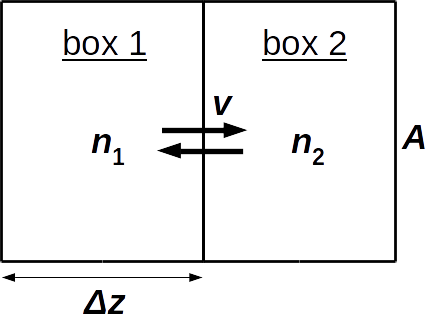
\includegraphics[width=5.5cm]{box2.png}\\[-5mm]
\caption{Diffusive mixing between two boxes.}
\label{2boxes}
\end{figure}

\section{What is mixing, and what is diffusion?}

Let's assume we have two identical boxes of length $\Delta z$ with cross
section $A$ touching each other, see Fig.~\ref{2boxes}. The total 
number of a certain kind of molecules in one of those boxes is
\begin{equation}
  N = n\,A\,\Delta z
\end{equation} 
where $n\rm\ [cm^{-3}]$ is the molecular particle density. From the 3D hydro
model, we observe that matter goes up and down with some
average (e.g.\ root-mean-square) velocity $\rm[cm/s]$ as
\begin{equation}
  v = v_{z,\rm rms} = \sqrt{\langle v_z^2 \rangle_t} 
                   = \sqrt{\langle v_z^2 \rangle_{\rm vol}}
\end{equation}
which either requires some kind of long-term average over time $t$ or
a spatial average over some suitably large volume. But there is no
bulk motion, otherwise it's an advection problem! We are talking here
about a mixing/diffusion problem, i.e. $\langle v_z \rangle_t =
\langle v_z \rangle_{\rm vol} = 0$.

Because of the random mixing motions, molecules will go from box~1 to
box~2 and vice versa. The associated mean particle fluxes $\rm[cm^{-2}s^{-1}]$ 
through the contact area $A$ are
\begin{eqnarray}
  j_1 = n_1\,v &\quad\quad& \mbox{rightwards}\\ 
  j_2 = n_2\,v &\quad\quad& \mbox{leftwards.}
\end{eqnarray}
The change of the total number of molecules $N_1$ in the left box is
\begin{eqnarray}
  dN_1 &=& -j_1\,A\,dt + j_2\,A\,dt = (n_2-n_1)\,v\,A\,dt \\
\Rightarrow
  \frac{dn_1}{dt} &=& \frac{n_2-n_1}{\Delta z}\,v
                 \;\;\to\;\; -\frac{\partial n}{\partial z}\,v
\end{eqnarray}

\paragraph{Diffusion with rate equations:}
The problem can be re-formulated with rate constants
$R=v/\Delta z \rm\,[1/s]$, like a chemist would do
\begin{eqnarray}
  \frac{dn_1}{dt} &=& -n_1 R + n_2 R \label{dn1}\\
  \frac{dn_2}{dt} &=& -n_2 R + n_1 R
\end{eqnarray}

\paragraph{The mixing timescale:}
Let's assume box~1 is full, and box~2 initially has none of those molecules. 
How long would it take to empty box~1? From Eq.~(\ref{dn1}), with
$n_2\to 0$, we find $n_1(t) = n_1(0) \exp(-t/\tau_{\rm mix})$ where
\begin{equation}  
  \boxed{\tau_{\rm mix} = \frac{1}{R} = \frac{\Delta z}{v}}
  \label{tmix1}
\end{equation}
The same result is obtained when considering the right box (index 2).
In {\tt static\_weather}, we replenish all distant boxes as
\begin{equation}
  \frac{dn_2}{dt} = \frac{n_1-n_2}{\tau_{\rm mix}}
  \label{ansatz}
\end{equation}
where index 1 refers to the ``full'' box which ultimately provides the
supply of fresh condensible material at some distance. Solving that
mixing ansatz (Eq.~\ref{ansatz}) for the mixing timescale results in 
\begin{equation}
  {\tau_{\rm mix}} = \frac{n_1-n_2}{\frac{dn_2}{dt}}
                  = \frac{n_1-n_2}{-n_2 R + n_1 R}
                  = \frac{1}{R}
\end{equation}
without having to assume anything for $n_1$ or $n_2$.

\section{A linear chain of boxes}

\begin{figure}[h!]
\centering
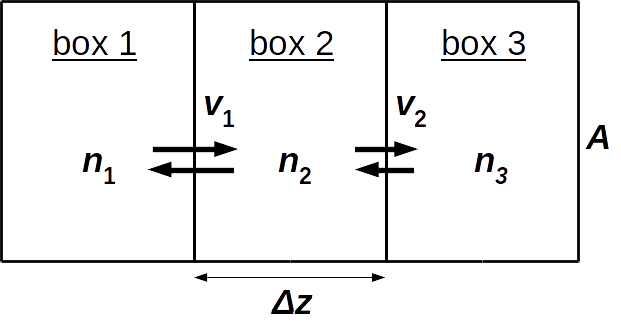
\includegraphics[width=8cm]{box3.png}\\[-5mm]
\caption{Diffusive mixing between three boxes.}
\label{3boxes}
\end{figure}

\noindent Let us now repeat the same thought experiment for 3 boxes in
a row as sketched in Fig.~\ref{3boxes}. The rate equations in this case, with
$R_1=v_1/\Delta z$ and $R_2=v_2/\Delta z$ are
\begin{eqnarray}
  \frac{dn_1}{dt} &=& -n_1 R_1 + n_2 R_1 \\
  \frac{dn_2}{dt} &=&  n_1 R_1 - n_2 (R_1+R_2) + n_3 R_2\label{dn2}\\ 
  \frac{dn_3}{dt} &=& -n_3 R_2 + n_2 R_2
\end{eqnarray}
Closer inspection of Eq.~(\ref{dn2}) shows the analogy to Fick's laws
\begin{eqnarray}
  \frac{dn_2}{dt} &=& \frac{n_1-n_2}{\Delta z}\,v_1 
                    + \frac{n_3-n_2}{\Delta z}\,v_2\\
  &\to& \frac{\partial}{\partial z}
      \left(\frac{\partial n}{\partial z}\,v\right)\Delta z
  \;=\; \frac{\partial}{\partial z}
      \left(D\,\frac{\partial n}{\partial z}\right) \ ,
\end{eqnarray}
where we find the diffusion constant $\rm[cm^2/s]$ (velocity $\times$
length) to be
\begin{equation}
  \boxed{D = v\,\Delta z}
  \label{D}
\end{equation}
The meaning of $\Delta z$ is a bit special in Eq.~(\ref{D}). The
mixing motions typically have a certain intrinsic range $\ell$, before the
incoming particles actually have an effect on the concentration in the
box.  When $\Delta z\ll\ell$, those particles simply rush through,
there is no time to mix with the ambient gas in the box. In the
opposite case, when $\Delta z\gg\ell$, those particles only enrich the
regions close to the surface $A$, but not in the entire box, the
concentration gradient on the box is substantial, and that
local enhancement at the surface should actually be taken into account when we
determine the flux backwards to the originating cell, which we do
not. Therefore, the only box thickness where the local Eq.~(\ref{D})
actually works fine is when
\begin{equation} 
  \mbox{Diffusion:}\quad\quad \Delta z \approx \ell \ .
\end{equation}
Indeed, when determining diffusion constants, we must always make some
kind of assumption about $\ell$, for example $\ell\sim$ the mean free
path for gas-kinetic diffusion, or $\ell\sim H_p$ for convective
mixing, where $H_p$ is the scale height.

However, for our ``global mixing approach'', we actually do not need
such an assumption. To find the mixing timescale $\tau_{\rm mix}$ for the
3-box experiment, we assume that the concentration $n_2$ in the
sandwich box 2 adjusts quickly to $n_1$ and $n_3$. Setting the time
derivative in Eq.~(\ref{dn2}) to zero we find
\begin{equation}
  n_2 = \frac{n_1 R_1 + n_3 R_2}{R_1+R_2} 
  \label{n_2}
\end{equation}
Generalising the derivation of $\tau_{\rm mix}$ from the 2-box
experiment, 
\begin{equation}
  \tau_{\rm mix}^{-1} = -\frac{1}{n_1}\frac{dn_1}{dt} 
                    = -\frac{1}{n_1}\Big(-n_1 R_1 + n_2 R_1\Big)
\end{equation}
and using Eq.~(\ref{n_2}) we find
\begin{equation}
  \tau_{\rm mix} = \frac{R_1 + R_2}{R_1 R_2}
                  \;\frac{1}{1-n_3/n_1}  \ ,
\end{equation}
which, in the limiting case of $n_3\to 0$, results in
\begin{equation}
  \boxed{\tau_{\rm mix} \;\to\; \frac{1}{R_1} + \frac{1}{R_2}
  \;=\; \frac{\Delta z}{v_1} + \frac{\Delta z}{v_2}} \ .
  \label{tmix2}
\end{equation}
Again, the same result is obtained when considering the right box
(index 3) and using Eq.~(\ref{n_2})
\begin{equation}
  {\tau_{\rm mix}} = \frac{n_1-n_3}{\frac{dn_3}{dt}}
                  = \frac{n_1-n_3}{-n_3 R_2 + n_2 R_2}
                  = \frac{\Delta z}{v_1} + \frac{\Delta z}{v_2} \ .
\end{equation}
This thought experiment can be extended to a linear chain of boxes of 
arbitrary length $K$. For each chain length, we consider $n_1$ and
$n_K$ to be given and assume that $n_2\,...\,n_{K-1}$ can be calculated in their
stationary limits. This is similar to the {\it Maxwell daemon} in
nucleation theory, who would always collect the large clusters, break
them up into monomers, and return them this way back to the gas phase.
Here, we need a daemon who makes
sure that $n_K$ stays small, and $n_1$ stays large. That deamon would
quickly transport the molecules arriving in the right box back to the
left box, to create a stationary problem with constant diffusive fluxes
through all interface areas. In our case, the deamon is dust
  formation and settling, causing a stationary situation.

Assuming $n_K \to 0$, the result is\footnote{I checked 4 boxes and 5
  boxes with Mathematica}
\begin{equation}
  \boxed{\tau_{\rm mix} \;=\; 
  \frac{1}{R_1} + \frac{1}{R_2} + ... + \frac{1}{R_{K-1}}
  \;\;\;=\;\;\; 
  \frac{\Delta z}{v_1} + \frac{\Delta z}{v_2} + ... + \frac{\Delta z}{v_{K-1}}}
  \label{tmix3}
\end{equation}
The same result is obtained for the mixing timescale of the right box
\begin{equation}
  {\tau_{\rm mix}} = \frac{n_1-n_K}{\frac{dn_K}{dt}}
   = \ldots 
   = \frac{\Delta z}{v_1} + \frac{\Delta z}{v_2} + 
     ... + \frac{\Delta z}{v_{K-1}} \ .
\end{equation}
In the limiting case $\Delta z\to 0$, the final result is
\begin{equation}
  \boxed{
  \tau_{\rm mix}(z) \;=\, \int_0^z \frac{1}{v(z')}\;dz'}
  \label{final}
\end{equation}
which shows that the result is independent of the choice 
of $\Delta z$ (disregarding here the uncertainties in
the actual numerical computation of that integral).


\newpage
This result makes a lot of sense to me:
\begin{itemize}
\item Equation (\ref{final}) states an expression for $\tau_{\rm mix}$
  that {\it matches its definition and use}. It is the replenishment timescale
  in consideration of a distant supply. 
\item The mixing timescale is monotonic increasing with $z$, i.e. it
  always takes longer to replenish an atmospheric layer which is
  higher above the ground.
\item There can be a bottleneck. If there is a region between 0 and
  $z$ where $v(z')$ is very slow, all regions above that region
  should indeed receive very little mixing supply.  This is likely to cause some
  numerical problems when trying to evaluate the integral, as locally,
  there might be a point where $v$ is very close to zero.
\item If $v=\rm const$, Eq.~(\ref{tmix3}) agrees with the 2-box result
  (Eq.~\ref{tmix1}) and the 3-box result (Eq.~\ref{tmix2}), namely
  $\tau_{\rm mix}(z)=z/v\quad(\beta=1$).
\end{itemize}

\bibliographystyle{chicagon}
\bibliography{references}

\end{document}
